\chapter{Results}
In this chapter we present the outcome of using CNN's for recovering images from compressed measurements. First, we present the alpha network and its performance using both learning approaches: supervised and unsupervised. We present the training, test and validation error for the dataset \ref{LFWTech}. Afterwards, we also show four images from the test dataset and compare them against the ground truth in terms of PSNR and SSIM. The same data can expected for the beta network. Finally, we present the time measurement that our approach need for fully reconstructing an image.  

\section{Alpha Network}
The alpha network was describe in section \ref{CHpateralphanet}. It is smaller than the beta network and in the following we show its performance.
\subsection{Supervised training}
For supervised learning we train the network using compressed measurements generated with the matrix $\Phi$. Figure \ref{fig:alphaSupValidPSNR} shows the training of the network for 100 epochs. The red solid line represents the PSNR on the whole training dataset whereas the red doted line represents the PSNR of the validation dataset. As it can been seen the error on the validation set is not as good as the training error but it is close to what is consider to prevent overfitting. Figure \ref{fig:alphaSupValidPSNR} is the progress on the test dataset over each epoch. Even, thought the difference is of almost  
\begin{figure}[tb] 
\centering 
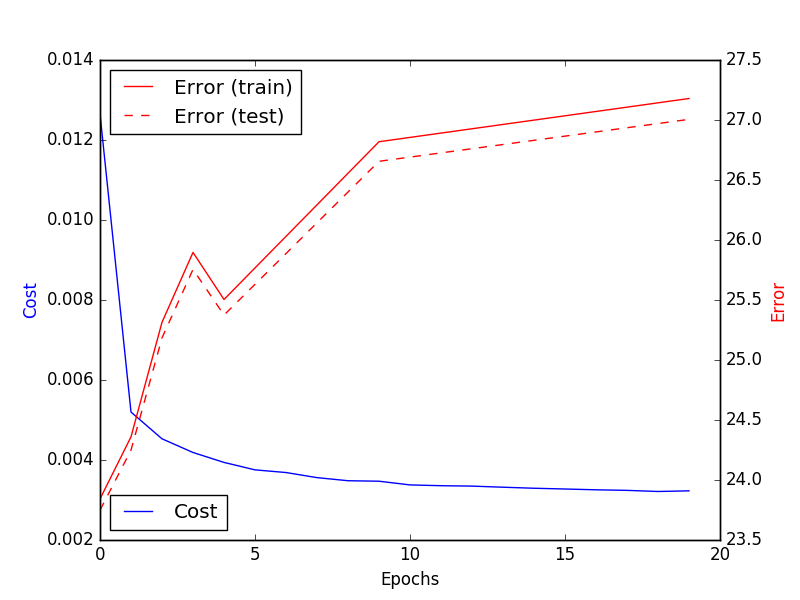
\includegraphics[scale=0.6]{alphaSup_PSNR_VALID_SET.png} 
\caption[PSNR validation progress during training of supervised alpha network]{PSNR progress over each epoch}
\label{fig:alphaSupValidPSNR} 
\end{figure}  

\begin{figure}[tb] 
\centering 
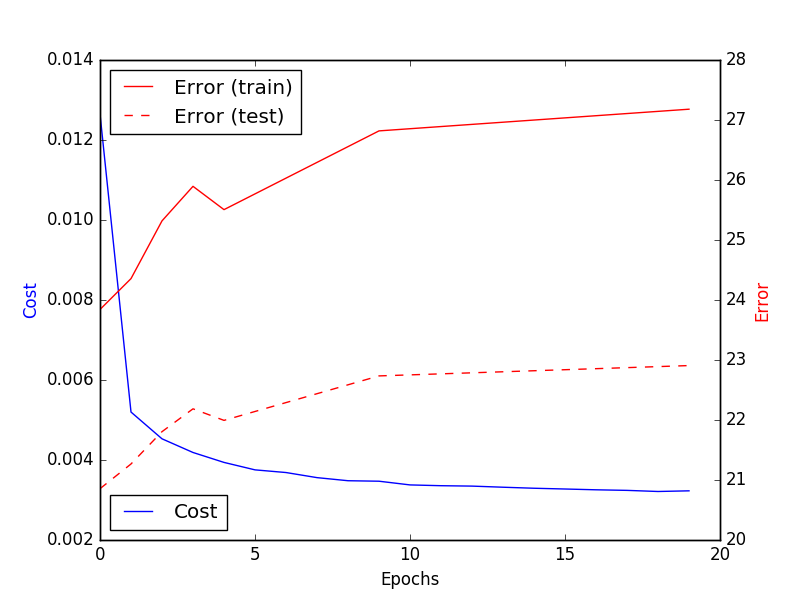
\includegraphics[scale=0.6]{alphaSup_PSNR_TEST_SET.png} 
\caption[PSNR testing progress during training of supervised alpha network]{PSNR progress over each epoch}
\label{fig:alphaSupTestPSNR} 
\end{figure}  

\begin{figure}[tb] 
\centering 
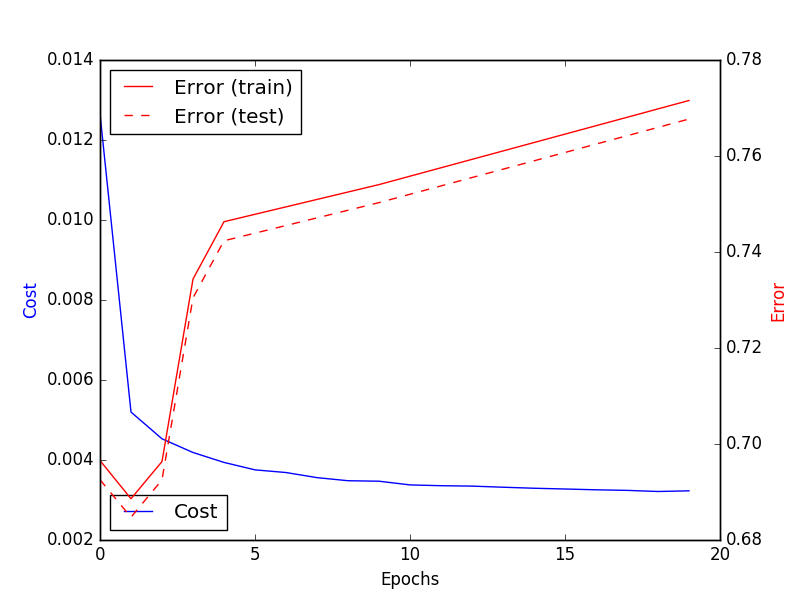
\includegraphics[scale=0.6]{alphaSup_SSIM_VALID_SET.png} 
\caption[SSIM validation progress during training of supervised alpha network]{SSIM progress over each epoch}
\label{fig:alphaSupValidSSIM} 
\end{figure}  

\begin{figure}[tb] 
\centering 
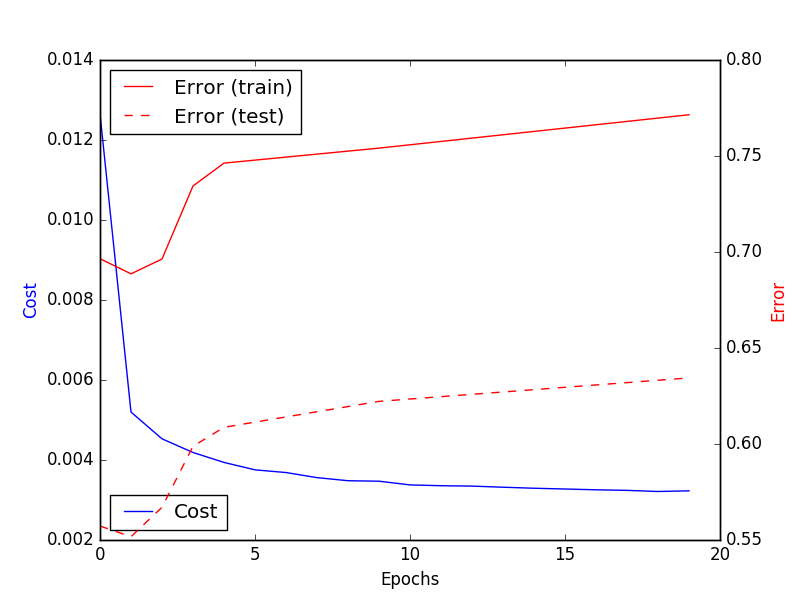
\includegraphics[scale=0.6]{alphaSup_SSIM_TEST_SET.png} 
\caption[SSIM testing progress during training of supervised alpha network]{SSIM progress over each epoch}
\label{fig:alphaSupTestSSIM} 
\end{figure}  


\subsection{Unsupervised training}

\begin{figure}[tb] 
\centering 
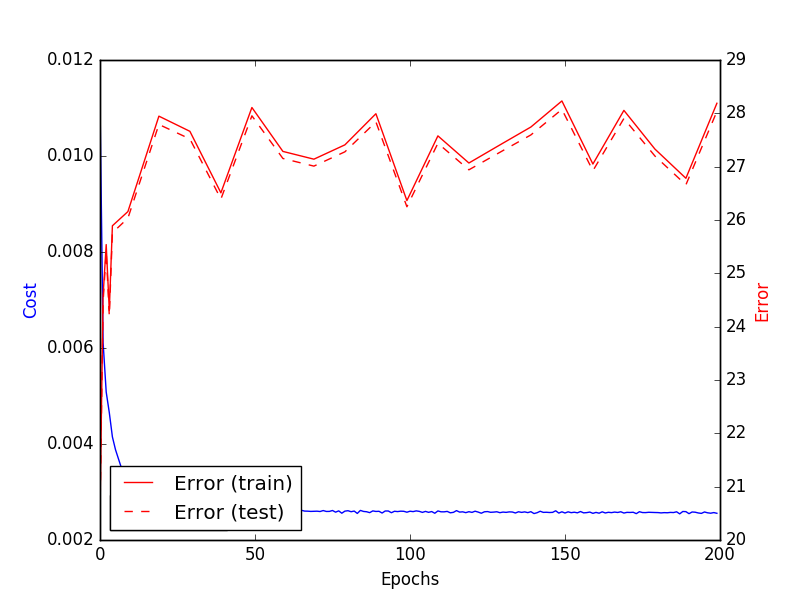
\includegraphics[scale=0.6]{alphaUnsup_PSNR_VALID_SET.png} 
\caption[PSNR validation progress during training of supervised alpha network]{PSNR progress over each epoch}
\label{fig:alphaUnsupValidPSNR} 
\end{figure}  

\begin{figure}[tb] 
\centering 
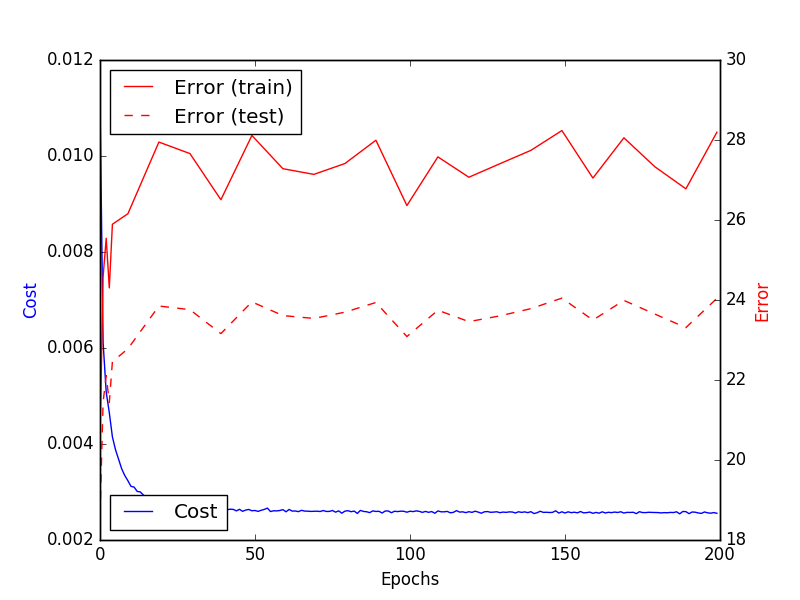
\includegraphics[scale=0.6]{alphaUnsup_PSNR_TEST_SET.png} 
\caption[PSNR testing progress during training of supervised alpha network]{PSNR progress over each epoch}
\label{fig:alphaUnsupTestPSNR} 
\end{figure}  

\begin{figure}[tb] 
\centering 
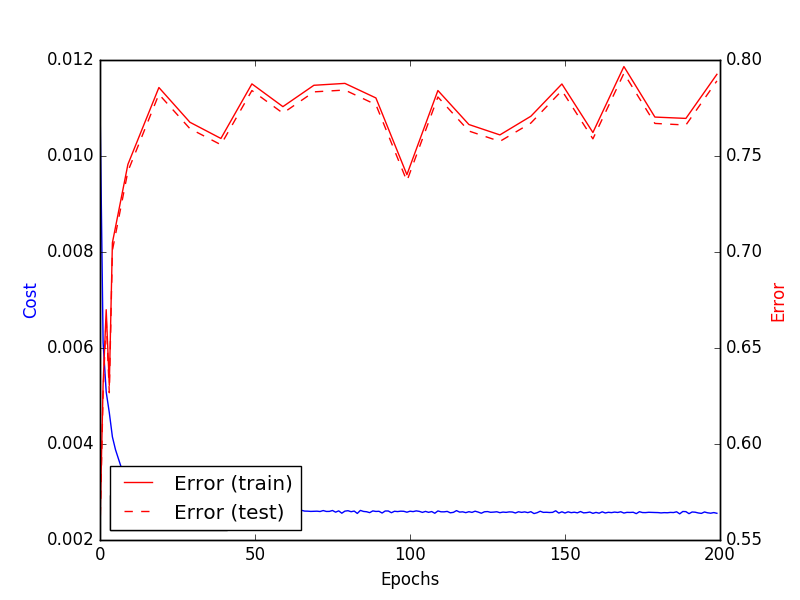
\includegraphics[scale=0.6]{alphaUnsup_SSIM_VALID_SET.png} 
\caption[SSIM validation progress during training of supervised alpha network]{SSIM progress over each epoch}
\label{fig:alphaUnsupValidSSIM} 
\end{figure}  

\begin{figure}[tb] 
\centering 
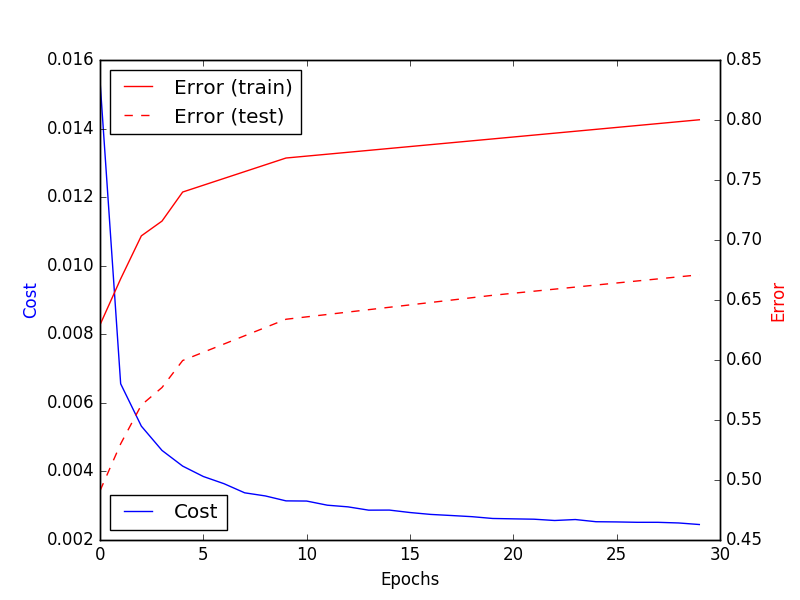
\includegraphics[scale=0.6]{alphaUnsup_SSIM_TEST_SET.png} 
\caption[SSIM testing progress during training of supervised alpha network]{SSIM progress over each epoch}
\label{fig:alphaUnsupTestSSIM} 
\end{figure}  

\section{Beta Network}

\subsection{Supervise training}
\begin{figure}[tb] 
\centering 
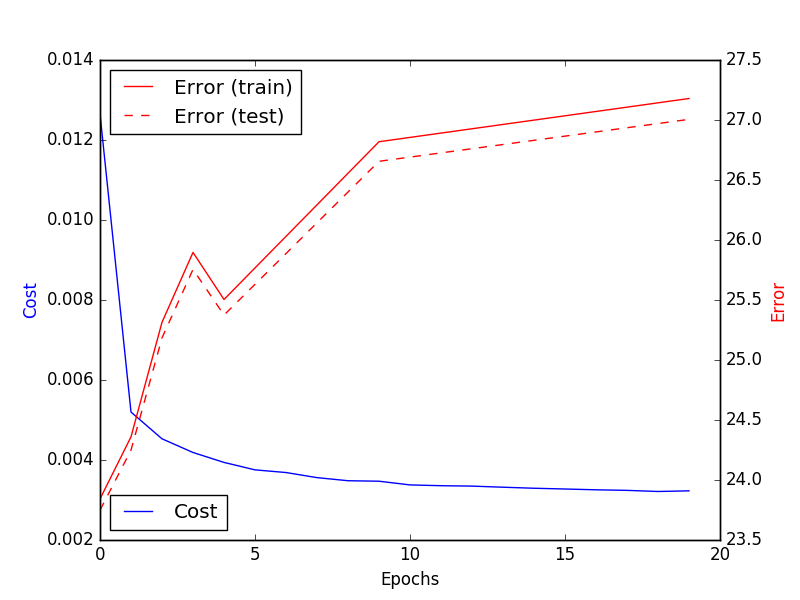
\includegraphics[scale=0.6]{betaSup_PSNR_VALID_SET.png} 
\caption[PSNR validation progress during training of supervised alpha network]{PSNR progress over each epoch}
\label{fig:betaSupValidPSNR} 
\end{figure}  

\begin{figure}[tb] 
\centering 
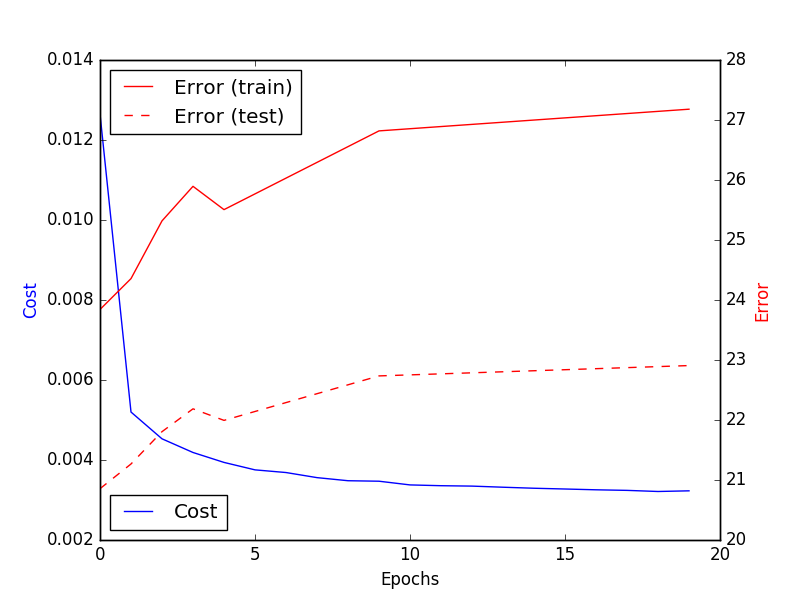
\includegraphics[scale=0.6]{betaSup_PSNR_TEST_SET.png} 
\caption[PSNR testing progress during training of supervised alpha network]{PSNR progress over each epoch}
\label{fig:betaSupTestPSNR} 
\end{figure}  

\begin{figure}[tb] 
\centering 
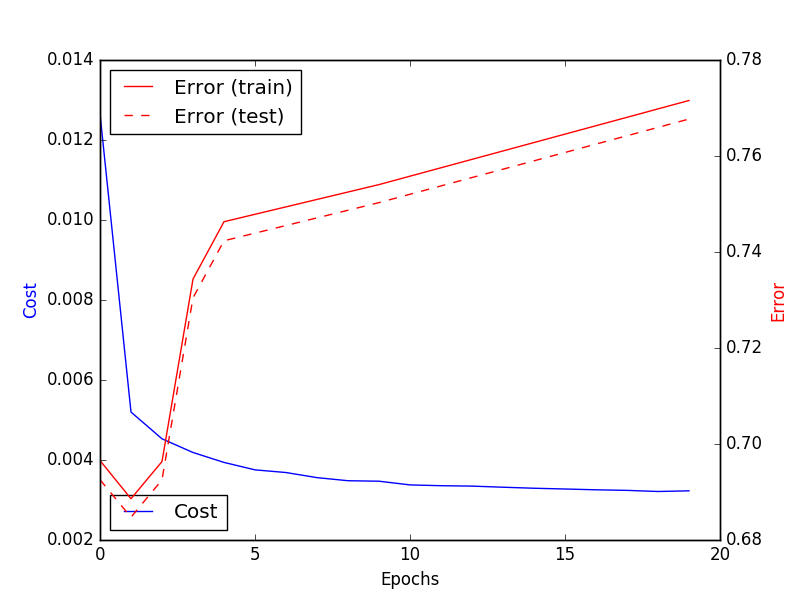
\includegraphics[scale=0.6]{betaSup_SSIM_VALID_SET.png} 
\caption[SSIM validation progress during training of supervised alpha network]{SSIM progress over each epoch}
\label{fig:betaSupValidSSIM} 
\end{figure}  

\begin{figure}[tb] 
\centering 
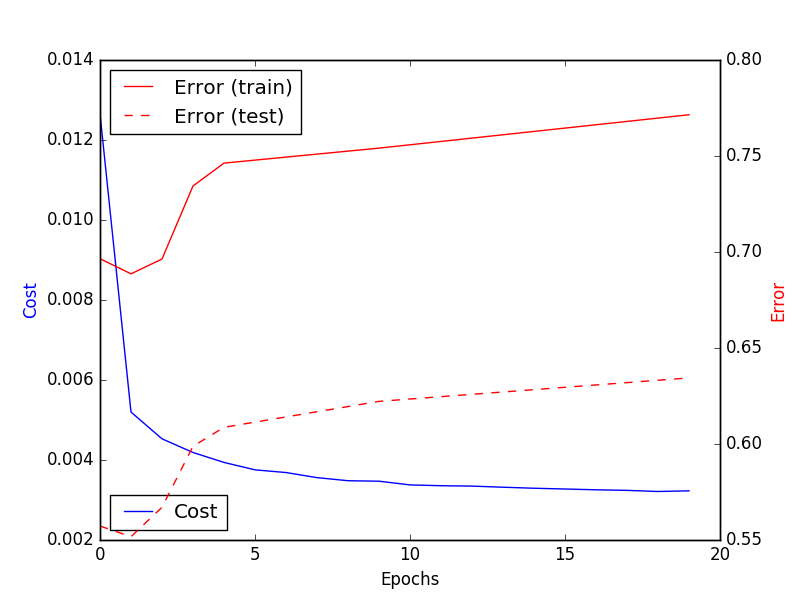
\includegraphics[scale=0.6]{betaSup_SSIM_TEST_SET.png} 
\caption[SSIM testing progress during training of supervised alpha network]{SSIM progress over each epoch}
\label{fig:betaSupTestSSIM} 
\end{figure}  

\subsection{Unsupervised training}

\begin{figure}[tb] 
\centering 
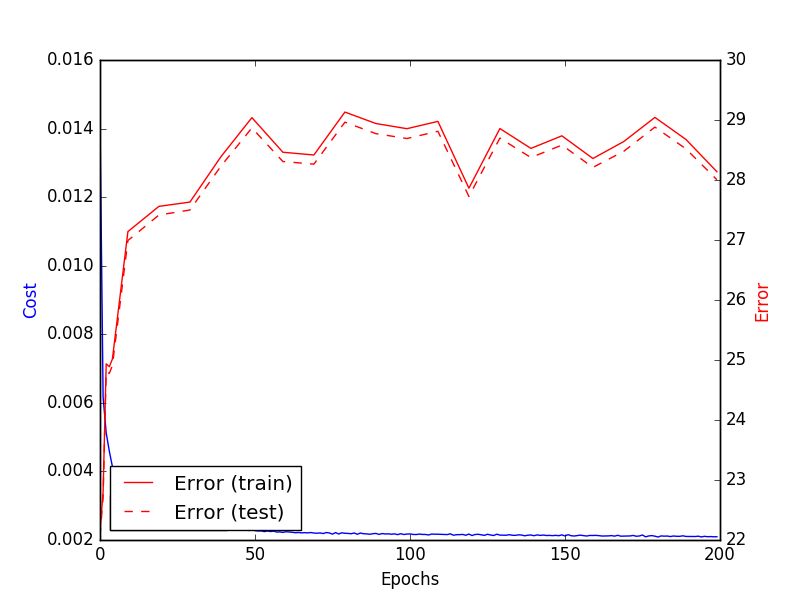
\includegraphics[scale=0.6]{betaUnsup_PSNR_VALID_SET.png} 
\caption[PSNR validation progress during training of supervised alpha network]{PSNR progress over each epoch}
\label{fig:betaUnsupValidPSNR} 
\end{figure}  

\begin{figure}[tb] 
\centering 
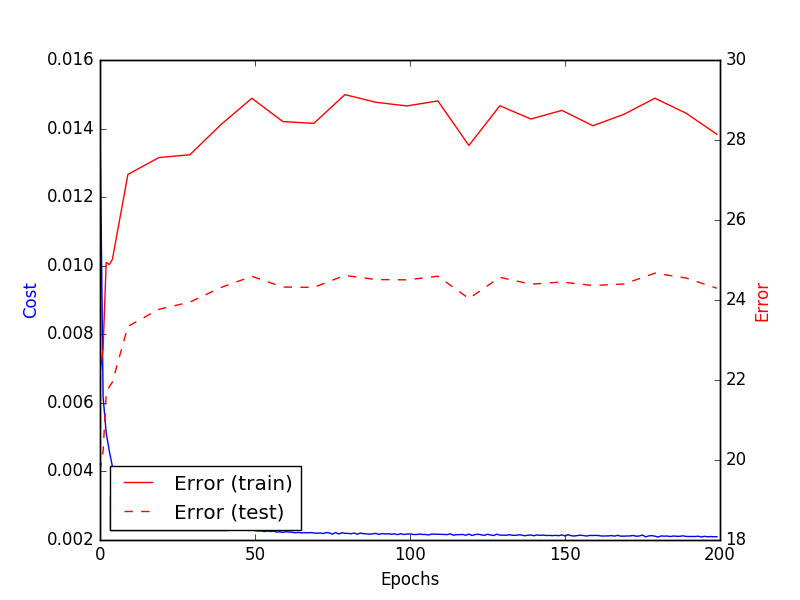
\includegraphics[scale=0.6]{betaUnsup_PSNR_TEST_SET.png} 
\caption[PSNR testing progress during training of supervised alpha network]{PSNR progress over each epoch}
\label{fig:betaUnsupTestPSNR} 
\end{figure}  

\begin{figure}[tb] 
\centering 
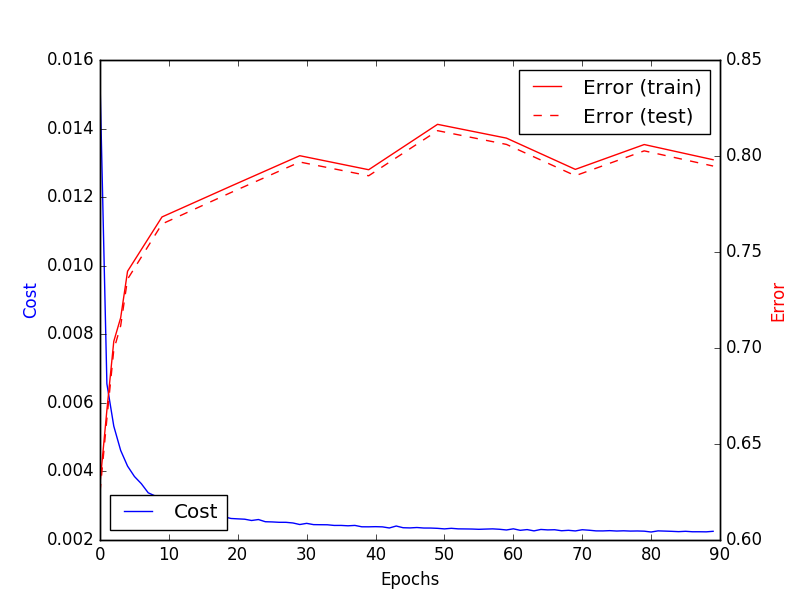
\includegraphics[scale=0.6]{betaUnsup_SSIM_VALID_SET.png} 
\caption[SSIM validation progress during training of supervised alpha network]{SSIM progress over each epoch}
\label{fig:betaUnsupValidSSIM} 
\end{figure}  

\begin{figure}[tb] 
\centering 
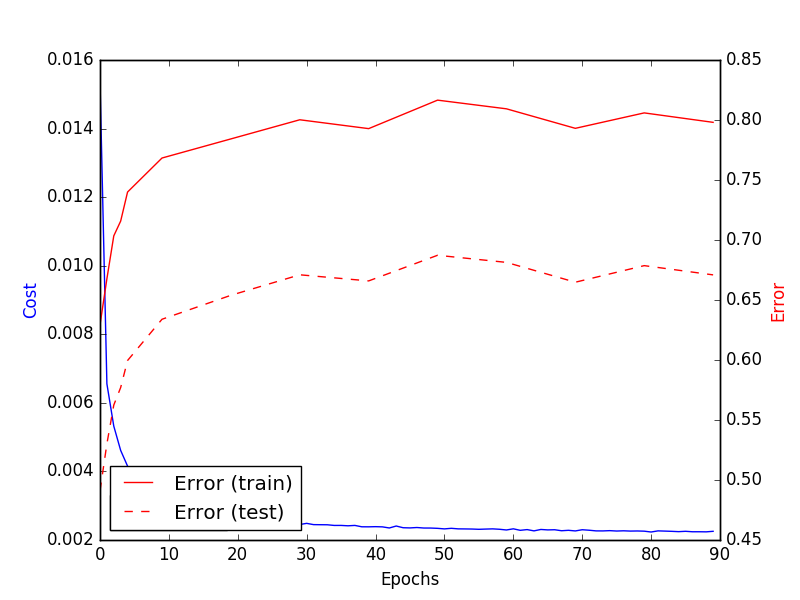
\includegraphics[scale=0.6]{betaUnsup_SSIM_TEST_SET.png} 
\caption[SSIM testing progress during training of supervised alpha network]{SSIM progress over each epoch}
\label{fig:betaUnsupTestSSIM} 
\end{figure}  
